% Préambule commun aux manuels d'Anticythere3D (français et anglais), au
% format maison des PDF : Latin Modern, titres sans empattement colorés,
% encadrés tcolorbox typés, icônes fontawesome, page de garde avec le logo.
% Compilation : ./compiler.sh (deux passes par langue, temporaires supprimés).
\documentclass[11pt,a4paper]{article}
\usepackage[utf8]{inputenc}
\usepackage[T1]{fontenc}
\usepackage{lmodern}
\usepackage{microtype}
\usepackage[a4paper,left=2.2cm,right=2.2cm,top=2.4cm,bottom=2.2cm,headheight=24pt]{geometry}
\usepackage{graphicx}
\usepackage[table]{xcolor}
\usepackage[most]{tcolorbox}
\usepackage{enumitem}
\usepackage{booktabs}
\usepackage{array}
\usepackage{tabularx}
\usepackage{amsmath}
\usepackage{amssymb}
\usepackage[nobottomtitles*]{titlesec}
\usepackage{needspace}
\usepackage{fancyhdr}
\usepackage{fontawesome5}
\usepackage{etoolbox}
\DeclareUnicodeCharacter{00B0}{\ifmmode^\circ\else\textdegree\fi}
\DeclareUnicodeCharacter{2192}{\ensuremath{\rightarrow}}
\DeclareUnicodeCharacter{2212}{\ensuremath{-}}

% Couleurs maison, et celles du programme (logo : nuit et bronze ; fond de la
% vue 3D : parchemin)
\definecolor{sky}{HTML}{1C6DB4}
\definecolor{skyl}{HTML}{E8F1F9}
\definecolor{alert}{HTML}{B5382B}
\definecolor{alertl}{HTML}{FBEAE7}
\definecolor{sapin}{HTML}{2C7A55}
\definecolor{sapinl}{HTML}{E4F2EA}
\definecolor{nuit}{HTML}{1C2A42}
\definecolor{bronze}{HTML}{A87C30}
\definecolor{bronzel}{HTML}{F8F0DD}
\definecolor{parchemin}{HTML}{F5F0E6}
\definecolor{summit}{HTML}{6B7A8F}
\definecolor{ink}{HTML}{1C2433}
\definecolor{lightblue}{HTML}{DCE8F4}
% les sept trains : valeurs exactes de anticythere/layout.py (COLORS)
\definecolor{trinput}{HTML}{DE6910}
\definecolor{trmoon}{HTML}{0D59C1}
\definecolor{tranomaly}{HTML}{8E1700}
\definecolor{trmetonic}{HTML}{1D9594}
\definecolor{trcallippic}{HTML}{786F4C}
\definecolor{trsaros}{HTML}{841959}
\definecolor{trexeligmos}{HTML}{B66CCD}
\newcommand{\pastille}[1]{\textcolor{#1}{\rule[-0.6mm]{9mm}{3.4mm}}}
\AtBeginDocument{\color{ink}}

\titleformat{\section}
  {\Large\bfseries\sffamily\color{sky}}
  {\makebox[1.6em][l]{\thesection}}{0.3em}{}
  [{\vspace{1pt}\color{sky!35}\titlerule[1.3pt]}]
\titlespacing*{\section}{0pt}{16pt}{8pt}
\titleformat{\subsection}{\large\bfseries\sffamily\color{alert}}{\thesubsection}{0.5em}{}
\pretocmd{\section}{\needspace{12\baselineskip}}{}{}
\pretocmd{\subsection}{\needspace{16\baselineskip}}{}{}
\widowpenalty=10000
\clubpenalty=10000
\raggedbottom
\setlength{\parindent}{0pt}
\setlength{\parskip}{6pt}
\setlist[enumerate]{itemsep=3pt,leftmargin=7mm}
\setlist[itemize]{itemsep=2pt,leftmargin=6mm}

\pagestyle{fancy}
\fancyhf{}
\renewcommand{\headrulewidth}{0.4pt}
\renewcommand{\headrule}{\hbox to\headwidth{\color{sky!40}\leaders\hrule height \headrulewidth\hfill}}
\fancyfoot[C]{\sffamily\small\color{summit}\thepage}
\renewcommand{\sectionmark}[1]{\markboth{#1}{}}

\newcommand{\menu}[1]{\textsf{\textbf{\textcolor{nuit}{#1}}}}
\newcommand{\touche}[1]{\tcbox[on line,boxsep=0pt,left=2pt,right=2pt,top=1.5pt,bottom=1.5pt,
  colback=white,colframe=summit,boxrule=0.5pt,arc=1.5pt]{\footnotesize\textsf{#1}}}
\newcommand{\fichier}[1]{\texttt{\small #1}}

% Encadrés typés : jamais coupés avec une ligne isolée (3 lignes au moins de
% chaque côté d'une coupure), et précédés d'un contrôle de place.
\newcommand{\encadre}[5]{%
  \newtcolorbox{#1}[1][#5]{enhanced,breakable,colback=#2,colframe=#3,
    coltitle=white,fonttitle=\bfseries\sffamily\small,boxrule=0.9pt,arc=2.5pt,
    left=3mm,right=3mm,top=1.5mm,bottom=1.5mm,title={#4~~##1},
    before upper={\widowpenalties 4 10000 10000 10000 0 \clubpenalties 4 10000 10000 10000 0}}%
  \BeforeBeginEnvironment{#1}{\par\needspace{8\baselineskip}}}

% \capture[largeur]{fichier}{légende}
\newcommand{\capture}[3][1]{\par\needspace{10\baselineskip}\begin{center}%
  \begin{minipage}{#1\linewidth}\centering\setlength{\fboxsep}{0pt}\setlength{\fboxrule}{0.6pt}%
  \fcolorbox{summit!50}{white}{\includegraphics[width=\dimexpr\linewidth-1.3pt\relax]{#2}}\\[1.5mm]
  {\small\color{summit}#3}\end{minipage}\end{center}}
\graphicspath{{../captures/}{../}}

\usepackage[french]{babel}
\usepackage[colorlinks=true,linkcolor=sky,urlcolor=sky]{hyperref}
\hypersetup{pdftitle={Anticythere3D — manuel d'utilisation},pdfauthor={},pdfcreator={Anticythere3D}}
\encadre{astuce}{sapinl}{sapin}{\faLightbulb}{Bon à savoir}
\encadre{info}{skyl}{sky}{\faInfoCircle}{Pour comprendre}
\encadre{attention}{alertl}{alert}{\faExclamationTriangle}{Attention}
\fancyhead[L]{\sffamily\small\color{sky}\textbf{ANTICYTHERE3D — MANUEL}}
\fancyhead[R]{\sffamily\small\color{summit}\leftmark}
\newcommand{\versionapp}{1.4.0}


\begin{document}

\begin{titlepage}
\centering
\vspace*{1.2cm}

\includegraphics[width=3.4cm]{../logo_1024.png}\par
\vspace{6mm}
{\sffamily\Huge\bfseries\color{nuit} ANTICYTHERE3D\par}
\vspace{3mm}
{\sffamily\LARGE\color{ink} Simulateur de la machine d'Anticythère\par}
\vspace{2mm}
{\sffamily\large\color{summit} Manuel d'utilisation \textbullet{} version \versionapp\par}
\vspace{8mm}
\setlength{\fboxsep}{0pt}\fcolorbox{summit!50}{white}{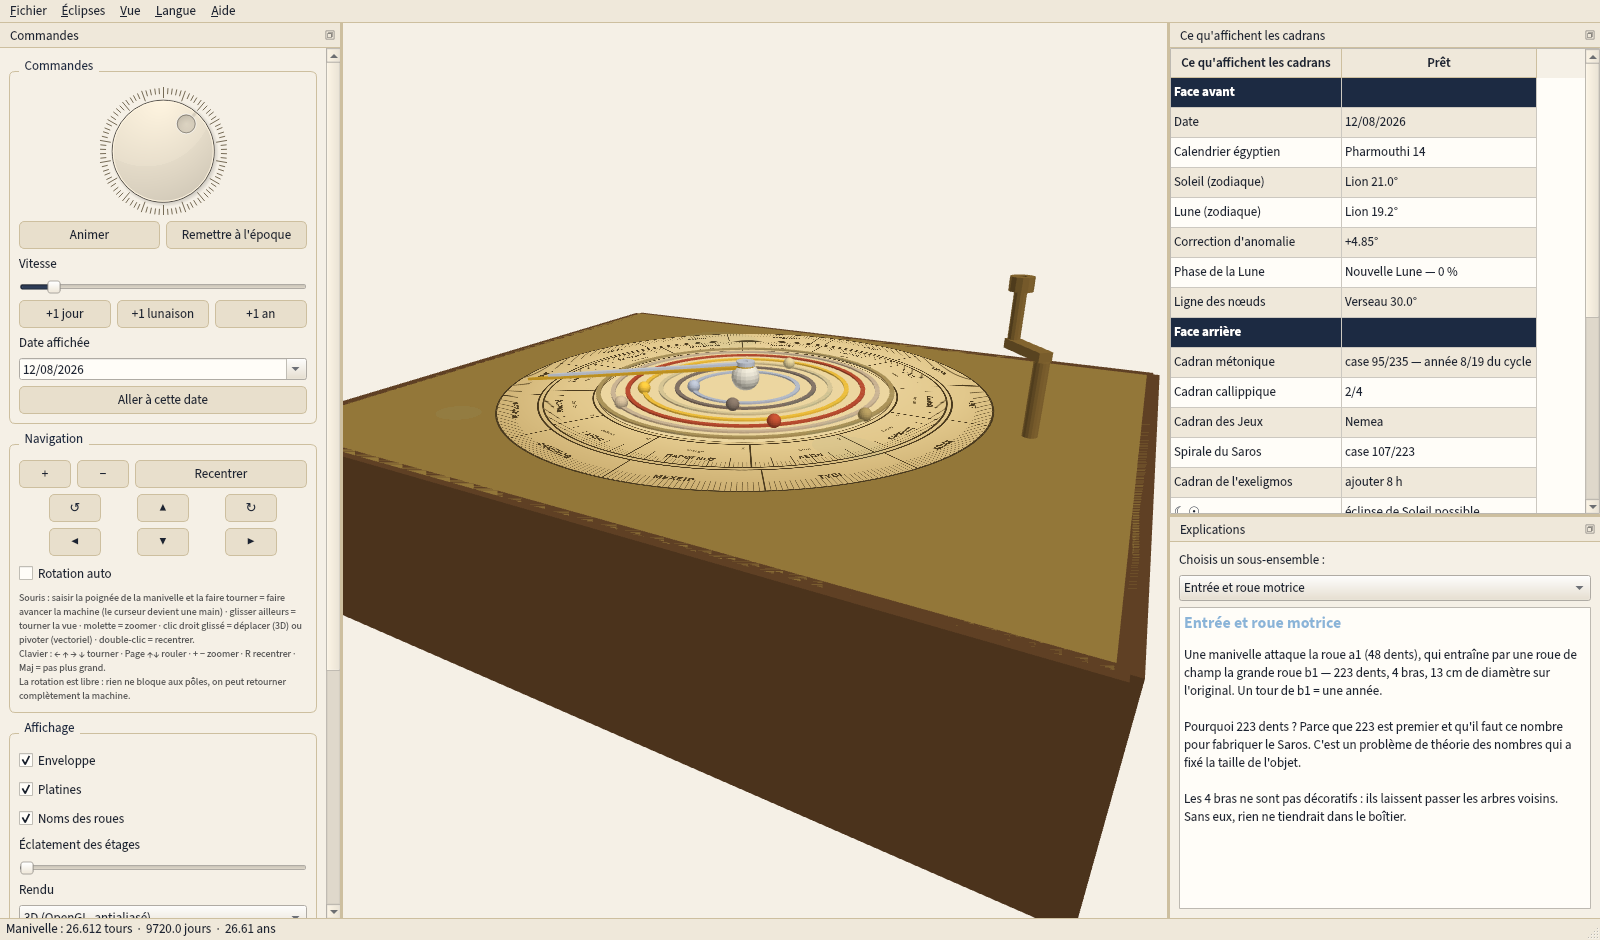
\includegraphics[width=0.86\textwidth]{fenetre-fr.png}}\par
\vspace{6mm}
\begin{tcolorbox}[enhanced,width=0.86\linewidth,colback=bronzel,colframe=bronze,arc=4pt,boxrule=1.1pt,left=5mm,right=5mm,top=2.5mm,bottom=2.5mm]
\sffamily\centering
Le premier calculateur astronomique connu, en état de marche :\\
\textbf{33 roues} \textbullet{} \textbf{15 arbres} \textbullet{} \textbf{2\,231 dents},
une seule manivelle.
\end{tcolorbox}
\vfill
{\footnotesize\color{summit}\sffamily Rapports exacts d'après Freeth \textit{et al.}, \textit{Nature} 2006 \&
2008, \textit{Scientific Reports} 2021\\[1mm]
Windows \textbullet{} macOS \textbullet{} Linux\par}
\end{titlepage}

\tableofcontents
\newpage

% =====================================================================
\section{Installer le programme}

\subsection{Le paquet prêt à l'emploi}

Les paquets sont sur la page \textbf{Releases} du dépôt
(\fichier{github.com/ARP273-ROSE/Anticythere3D/releases}). Chacun
\textbf{embarque son propre Python} : rien d'autre à installer, et aucun mot de
passe administrateur n'est demandé.

\begin{center}
\small
\renewcommand{\arraystretch}{1.25}
\begin{tabularx}{\textwidth}{@{}p{2.5cm}p{6.1cm}X@{}}
\toprule
\rowcolor{lightblue}\textbf{Système} & \textbf{Fichier} & \textbf{Installation} \\
\midrule
\textbf{Windows} & \fichier{Anticythere3D-Setup.exe} & lancer l'installeur ; il installe dans
le profil (\fichier{\%LOCALAPPDATA\%\textbackslash Programs}), sans droits d'administrateur \\
\textbf{macOS} Apple Silicon / Intel & \fichier{Anticythere3D-macos-arm64.dmg}\newline
\fichier{Anticythere3D-macos-x86\_64.dmg} & ouvrir l'image, glisser l'application dans
\menu{Applications} \\
\textbf{Linux} x86\_64 / ARM64 & \fichier{Anticythere3D-linux-x86\_64.tar.gz}\newline
\fichier{Anticythere3D-linux-arm64.tar.gz} & décompresser, lancer \fichier{./installer.sh} :
installation dans \fichier{\textasciitilde/.local/share}, entrée de menu, \textbf{sans sudo} \\
\bottomrule
\end{tabularx}
\end{center}

Ces noms sans numéro de version sont des liens permanents vers la dernière version ; la
page Releases propose aussi les mêmes fichiers numérotés, et un fichier
\fichier{SHA256SUMS} qui donne l'empreinte de chacun.

\begin{attention}[Paquets non signés]
\textbf{Windows} : « Windows a protégé votre ordinateur » — cliquer \menu{Informations
complémentaires} puis \menu{Exécuter quand même}, une seule fois. \textbf{macOS} : la
première fois, \textbf{clic droit} sur l'application → \menu{Ouvrir}, puis confirmer ; si
macOS refuse encore : \menu{Réglages Système → Confidentialité et sécurité → Ouvrir quand
même}.
\end{attention}

\subsection{La mise à jour se fait toute seule}

Sur les trois systèmes, le programme installé regarde, quelques secondes après son
ouverture, si une version plus récente est publiée. Si oui, il le propose, avec les
nouveautés dans la langue de l'interface ; on peut aussi le demander par
\menu{Aide → Rechercher des mises à jour…}. Seule une \textbf{petite archive de code}
est téléchargée ; sa taille et son empreinte sont vérifiées, elle est déballée à la place
de l'ancienne, puis le programme redémarre. Lancé depuis les sources, il ne remplace rien :
il propose la page de téléchargement (ou \fichier{git pull}).

\begin{info}[Si la mise à jour échoue]
Le message « un fichier de l'application est utilisé par un autre programme » signifie
qu'une autre copie du programme tourne. Fermez-la (ou redémarrez l'ordinateur) et
redemandez la mise à jour : la version en place reste intacte.
\end{info}

\subsection{Les rapports d'incident}

S'il plante, se fige ou refuse de démarrer, le programme peut le signaler lui-même à celui
qui le maintient. \textbf{Rien ne part sans accord} : la question est posée au premier
lancement, et la case \menu{Aide → Envoyer automatiquement les rapports d'incident} permet
de changer d'avis. \menu{Aide → Signaler un problème…} envoie un signalement écrit, avec vos
mots. Le rapport contient la version, le système et la trace de l'erreur ; ni fichier, ni
nom, ni chemin personnel. Sans réseau, il attend le démarrage suivant.

\subsection{Où vivent vos données}

Réglages, rapports et journal ne sont \textbf{jamais} rangés dans le dossier du programme,
puisque la mise à jour le remplace en entier :

\begin{center}
\begin{tabularx}{0.92\textwidth}{@{}lX@{}}
\toprule
\rowcolor{lightblue}\textbf{Système} & \textbf{Dossier des données} \\
\midrule
Windows & \fichier{\%LOCALAPPDATA\%\textbackslash Anticythere3D} \\
macOS & \fichier{\textasciitilde/Library/Application Support/Anticythere3D} \\
Linux & \fichier{\textasciitilde/.local/share/Anticythere3D} (ou \fichier{\$XDG\_DATA\_HOME}) \\
\bottomrule
\end{tabularx}
\end{center}

\subsection{Depuis les sources}

Il suffit d'avoir \textbf{Python 3.10 ou plus récent} (sous Windows, un double-clic sur
\fichier{launch.bat} fait tout). Le reste — y compris la 3D — est installé par le
programme lui-même au premier démarrage : \fichier{python run.py}.

\begin{astuce}[Ce qu'il installe, et où]
Quatre paquets : \fichier{PyQt6} (l'interface), \fichier{numpy} (la géométrie),
\fichier{pyqtgraph} et \fichier{PyOpenGL} (la vue 3D). Hors environnement virtuel,
l'installation se fait avec \fichier{-{}-user} : \textbf{rien n'est écrit dans les paquets
du système}. Sous Linux, s'il manque à Qt des bibliothèques système, le programme affiche
la commande exacte à lancer.
\end{astuce}

\begin{center}
\begin{tabularx}{0.95\textwidth}{@{}lX@{}}
\toprule
\rowcolor{lightblue}\textbf{Commande} & \textbf{Effet} \\
\midrule
\fichier{python run.py -{}-check} & vérifie dépendances, style, logo et manuels, puis sort \\
\fichier{python run.py -{}-no-install} & démarre sans rien installer \\
\fichier{python run.py -{}-lang en} & interface en anglais (défaut : langue du système) \\
\fichier{python run.py -{}-vector} & démarre en rendu vectoriel \\
\fichier{python run.py -{}-samples 16} & antialiasing plus poussé (défaut : 8) \\
\bottomrule
\end{tabularx}
\end{center}

\begin{attention}[Si la 3D ne démarre pas]
Sur une machine sans pilote OpenGL (serveur, machine virtuelle, bureau à distance),
\textbf{le programme ne plante pas} : il bascule tout seul en \emph{rendu vectoriel}, qui
montre les mêmes rotations sans dépendance graphique — et exporte en SVG et en PDF.
\end{attention}

% =====================================================================
\section{Prise en main en deux minutes}

\begin{enumerate}
  \item Ouvrez le programme. La machine apparaît \textbf{fermée}, comme on la trouverait sur
        une étagère : coffret de bois, façade de bronze gravée, aiguilles, manivelle sur le
        côté. Le programme parle la langue du système ; le menu \menu{Langue} permet de
        choisir le français ou l'anglais, et ce choix est retenu.
  \item Au premier lancement, une question : accepter ou non l'envoi automatique des
        rapports d'incident (voir plus haut).
  \item Faites avancer la machine : \textbf{saisissez la poignée de la manivelle} à la
        souris, sur le flanc, et faites-la tourner (le curseur devient une main) — ou tournez
        le \textbf{bouton rond} en haut à gauche, dont un tour complet vaut une année.
  \item Décochez \menu{Enveloppe} : le coffret disparaît et les 33 roues apparaissent, en
        train de tourner.
  \item Regardez le panneau de droite : il donne en permanence ce que lisait le propriétaire
        de la machine.
\end{enumerate}

\capture{ouvert-fr.png}{L'enveloppe retirée, au 12 août 2026 : les 33 roues, les 15 arbres
et les deux grandes roues à bras ($b_1$ devant, $e_3$ derrière). À droite, la Lune est nouvelle
et le panneau annonce une éclipse de Soleil possible — celle du jour même.}

\begin{astuce}[Une apparence qui ne change pas d'un ordinateur à l'autre]
Le programme impose son propre style (couleurs parchemin et bleu de nuit, police Source
Sans 3 livrée avec lui) : il garde le même aspect sous Windows, macOS et Linux, que le
système soit en thème clair ou sombre. Seule la mise à l'échelle de l'écran (125~\%,
150~\%…) reste celle du système.
\end{astuce}

% =====================================================================
\section{L'interface}

\subsection{Commandes}

\begin{center}
\begin{tabularx}{\textwidth}{@{}lX@{}}
\toprule
\rowcolor{lightblue}\textbf{Élément} & \textbf{Rôle} \\
\midrule
Poignée de la manivelle & dans la vue : la \textbf{seule} entrée de la machine, saisie à la
souris (voir ci-dessous) \\
Bouton rond & la même manivelle, démultipliée : un tour = une année \\
Animer / Pause & fait tourner la manivelle en continu \\
Vitesse & nombre de jours simulés par seconde \\
+1 jour / +1 lunaison / +1 an & avance d'un pas exact \\
Remettre à l'époque & ramène la machine à sa date de calage \\
Date affichée + Aller à cette date & saute directement à une date \\
\bottomrule
\end{tabularx}
\end{center}

\begin{info}[Pourquoi une seule entrée ?]
Parce que la machine réelle n'en a qu'une. Tout le reste — Soleil, Lune, phase, éclipses,
calendriers — n'est pas « calculé » séparément : ce sont des rapports d'engrenages, donc des
conséquences mécaniques du seul mouvement de la manivelle. C'est exactement ce que fait le
programme : aucune formule d'affichage, seulement des fractions de nombres de dents.
\end{info}

\subsection{Tourner la manivelle à la souris}

\capture{manivelle-fr.png}{Avant et après un tour de poignée : la date passe du 12/08 au
30/10/2026 (78,6 jours), la Lune passe de nouvelle à gibbeuse décroissante.}

\begin{enumerate}
  \item Amenez la souris sur la \textbf{poignée} (ou le bras) de la manivelle, sur le flanc
        droit du coffret : le curseur devient une \textbf{main ouverte}.
  \item Cliquez et gardez le bouton enfoncé : la main se ferme, la poignée est saisie.
  \item Décrivez un cercle autour de l'axe de la manivelle : la machine avance dans un sens,
        recule dans l'autre. Tous les cadrans suivent, et le bouton rond aussi.
\end{enumerate}

\begin{info}[Combien vaut un tour de poignée ?]
La manivelle porte la roue $a_1$ (48 dents), qui engrène la grande roue $b_1$ (223 dents).
Un tour de poignée fait donc tourner $b_1$ de $48/223$ de tour — et $b_1$ fait un tour par an :
\[
  1~\text{tour de poignée} = \frac{48}{223}~\text{année}
  \approx \frac{48}{223}\times 365{,}24 \approx 78{,}6~\text{jours},
\]
en sens contraire de $b_1$, comme deux roues qui s'engrènent. Il faut donc
$223/48 \approx 4{,}65$ tours de poignée pour une année.
\end{info}

Le geste est le même en \textbf{rendu vectoriel}, où la manivelle est dessinée sur la roue
$a_1$. Hors de la poignée, glisser fait toujours tourner la vue : on ne fait pas avancer la
machine par mégarde. La molette tournée \emph{au-dessus du bouton rond} fait aussi avancer la
machine.

\subsection{Navigation : zoomer, tourner, retourner}

\begin{center}
\begin{tabularx}{\textwidth}{@{}p{5.2cm}X@{}}
\toprule
\rowcolor{lightblue}\textbf{Geste} & \textbf{Effet} \\
\midrule
Glisser sur la poignée & tourner la manivelle (curseur en main) \\
Glisser ailleurs & faire tourner l'objet \\
Molette & zoomer vers l'avant, dézoomer vers l'arrière (zoom borné : on ne traverse pas la
machine) \\
Clic droit et glisser & déplacer (3D) ou pivoter (vectoriel) \\
Double-clic & recentrer \\
\touche{←} \touche{↑} \touche{→} \touche{↓} & tourner au clavier \\
\touche{Page ↑} / \touche{Page ↓} & rouler (3\textsuperscript{e} axe) \\
\touche{+} / \touche{−} & zoomer / dézoomer \\
\touche{R} & recentrer \\
\touche{Maj} enfoncée & pas de rotation plus grand \\
\touche{Espace} & animer / pause \\
\touche{F} / \touche{B} / \touche{I} & face avant / face arrière / vue de trois quarts \\
\touche{E} & liste des prochaines éclipses \\
\touche{F1} & ce manuel \\
\bottomrule
\end{tabularx}
\end{center}

\begin{astuce}[Rotation vraiment libre]
La caméra est pilotée par \emph{quaternion} et non par angles d'Euler : \textbf{rien ne bloque
aux pôles}. On peut passer au-dessus, continuer, et retourner complètement la machine.
\menu{Recentrer} (ou \touche{R}) ramène toujours exactement à la même vue de trois quarts,
quels qu'aient été les roulis précédents.
\end{astuce}

\subsection{Affichage}

\begin{center}
\begin{tabularx}{\textwidth}{@{}lX@{}}
\toprule
\rowcolor{lightblue}\textbf{Réglage} & \textbf{Effet} \\
\midrule
\textbf{Enveloppe} & montre ou retire le coffret et la façade (la manivelle reste, pour qu'on
puisse la saisir) \\
Platines & les deux plaques intérieures qui portent les arbres \\
Noms des roues & étiquette chaque roue avec son nombre de dents \\
Éclatement des étages & écarte les 16 plans d'engrènement le long des arbres \\
\textbf{Rendu} & 3D temps réel, ou vectoriel exportable \\
\textbf{Profil des dents} & triangulaire (antique) ou développante (moderne) \\
Mettre en évidence & n'éclaire qu'un sous-ensemble, estompe les autres \\
\bottomrule
\end{tabularx}
\end{center}

\begin{info}[Les deux profils de dents]
Les dents de la machine réelle sont des \textbf{triangles quasi équilatéraux}. Le rapport
\emph{moyen} est alors rigoureusement exact — c'est pour cela que l'instrument est juste —
mais le rapport \emph{instantané} oscille à chaque passage de dent. La \textbf{développante de
cercle}, inconnue des Grecs, est le seul profil qui donne un rapport constant à tout instant.
\end{info}

\subsection{L'éclatement des étages}

\capture{eclatement-fr.png}{Éclatement à 0, 50 et 100~\% : la pile s'étire le long des arbres,
aucune roue ne quitte son plan.}

Les 33 roues sont rangées sur \textbf{16 étages} : deux roues d'un même étage sont dans le même
plan et s'engrènent. Le curseur \menu{Éclatement des étages} fait passer l'écart entre deux
étages de 3,4~mm (machine montée) à 15,4~mm :
\begin{itemize}
  \item le \textbf{fond} reste en place et la pile s'étire vers l'avant ; la façade (cadrans,
        Cosmos, aiguilles, manivelle) avance avec le premier étage ;
  \item \textbf{aucune roue ne bouge dans son plan} ; celles qui s'engrènent restent face à
        face, et l'ordre des étages ne change jamais ;
  \item les \textbf{arbres s'allongent} avec la pile : aucune roue ne flotte ;
  \item en rendu vectoriel le curseur est grisé : l'éclatement s'y ferait dans l'axe de visée.
\end{itemize}

\begin{info}[Aucune pièce n'en traverse une autre]
La suite de tests vérifie, à six positions du curseur et pour 76 angles du porte-satellite
$e_3$, qu'aucune roue n'en pénètre une autre et qu'aucun arbre, \textbf{prolongé jusqu'à son
cadran}, ne traverse une roue. Ce contrôle a fait corriger deux défauts en version 1.3.1 :
l'arbre $o$ de l'aiguille callippique passait au travers de la roue $i_1$ de l'exeligmos (il a
été déplacé sur son cercle d'entraxe autour de $p$, entraxe exact conservé) ; les roues $k_1$,
$k_2$ du tenon-fente, qui tournent avec $e_3$, balayaient les arbres $b$ et $l$ (elles sont
maintenant juste devant $e_3$, qui les porte).
\end{info}

\capture[0.55]{arbre_o_callippique.png}{Le train callippique mis en évidence (machine éclatée,
vue de trois quarts arrière) : l'arbre $o$ descend jusqu'au cadran sans traverser aucune roue.}

\subsection{Les couleurs des sept trains}

Chaque sous-ensemble a sa couleur, dans la vue 3D, dans le rendu vectoriel et ses exports, et
dans la légende. \menu{Mettre en évidence} n'en éclaire qu'un :

\capture[0.62]{evidence-saros-fr.png}{Le train du Saros mis en évidence, les autres estompés.}

\begin{center}
\small
\begin{tabularx}{\textwidth}{@{}lllX@{}}
\toprule
\rowcolor{lightblue}\textbf{Couleur} & \textbf{Code} & \textbf{Train} & \textbf{Roues} \\
\midrule
\pastille{trinput} orange & \fichier{\#DE6910} & Entrée et roue motrice & $a_1$, $b_1$, $b_2$ \\
\pastille{trmoon} bleu & \fichier{\#0D59C1} & Train de la Lune & $b_3$, $c_1$, $c_2$, $d_1$, $d_2$, $e_1$, $e_2$, $e_5$, $e_6$ \\
\pastille{tranomaly} rouge sang & \fichier{\#8E1700} & Anomalie lunaire (tenon et fente) & $e_3$, $e_4$, $k_1$, $k_2$ \\
\pastille{trmetonic} bleu-vert & \fichier{\#1D9594} & Cycle métonique & $l_1$, $l_2$, $m_1$, $m_2$, $n_1$ \\
\pastille{trcallippic} kaki & \fichier{\#786F4C} & Cycle callippique & $n_2$, $p_1$, $p_2$, $o_1$ \\
\pastille{trsaros} framboise & \fichier{\#841959} & Saros (éclipses) & $m_3$, $f_1$, $f_2$, $g_1$ \\
\pastille{trexeligmos} lilas & \fichier{\#B66CCD} & Exeligmos & $g_2$, $h_1$, $h_2$, $i_1$ \\
\bottomrule
\end{tabularx}
\end{center}

\begin{info}[Une palette calculée, pas choisie à l'œil]
Les sept teintes sortent d'une optimisation (\fichier{anticythere/palette.py}) : écart de
couleur CIEDE2000 d'au moins 27,7 entre toutes en vision normale ; en deutéranopie et
protanopie simulées, au moins 19 entre trains qui se touchent et 12 entre tous ; contraste
d'au moins 3:1 sur le fond parchemin. Les tests vérifient ces seuils à chaque version.
\end{info}

\subsection{Le rendu vectoriel et les exports}

\capture{vectoriel-fr.png}{Rendu vectoriel de la face avant, avec sa légende : chaque dent est
une courbe, pas un pixel.}

Ce mode dessine les \textbf{dentures réelles} en courbes. Il sert à trois choses :
\begin{itemize}
  \item regarder le mécanisme à plat, sans occlusion ;
  \item exporter en \textbf{SVG} ou en \textbf{PDF A3} (\menu{Fichier}) — les fichiers ne
        contiennent aucune image bitmap : on peut imprimer en A0 ou zoomer sans fin ;
  \item fonctionner sur une machine dépourvue d'OpenGL.
\end{itemize}

Le menu \menu{Fichier} propose aussi une capture PNG de la fenêtre, l'export CSV du panneau
des cadrans et l'export \textbf{STL} des 33 roues, prêtes à imprimer en 3D (jeu de 0,15~mm et
alésage de 3,2~mm déjà appliqués, avec une nomenclature).

\capture[0.8]{enregistrer-fr.png}{La boîte d'enregistrement : un vrai explorateur, avec ses
raccourcis (dossier personnel, Bureau, Documents, Images, Téléchargements), l'arborescence, la
création de dossier et le filtre de type.}

\begin{astuce}[Sous Linux aussi, un vrai explorateur de fichiers]
Sous Linux, la boîte « native » passe souvent par un portail qui la réduit à une simple liste.
Le programme y impose donc la boîte complète de Qt, montrée ci-dessus, avec les emplacements
usuels dans la barre latérale et les supports montés (clés USB, disques). Sous Windows et
macOS, c'est la boîte du système, déjà complète.
\end{astuce}

% =====================================================================
\section{Ce qu'affichent les cadrans}

\subsection{Le panneau de report}

Le panneau de droite se détache (c'est une fenêtre à part entière) et donne :

\begin{center}
\small
\begin{tabularx}{\textwidth}{@{}lX@{}}
\toprule
\rowcolor{lightblue}\textbf{Ligne} & \textbf{Signification} \\
\midrule
Date & date grégorienne correspondant à la position de la manivelle \\
Calendrier égyptien & mois et jour du calendrier de 365 jours de la face avant \\
Soleil (zodiaque) & position du Soleil moyen — c'est aussi le pointeur de date \\
Lune (zodiaque) & position de la Lune, anomalie comprise \\
Correction d'anomalie & écart produit par le tenon-fente, au plus $\pm 6{,}58°$ \\
Phase de la Lune & nom de la phase et pourcentage éclairé \\
Ligne des n\oe uds & position des n\oe uds, qui décide des éclipses \\
Cadran métonique & case sur 235 et année sur 19 du cycle \\
Cadran callippique & quart sur 4 du cycle de 76 ans \\
Cadran des Jeux & jeu panhellénique de l'année \\
Spirale du Saros & case sur 223 \\
Cadran de l'exeligmos & correction horaire à ajouter : 0, 8 ou 16 heures \\
\textbf{Lune et Soleil} & annonce d'éclipse possible ou quasi certaine \\
Planètes & positions selon le modèle de Freeth \textit{et al.} (2021) \\
Écart machine / ciel réel & \textbf{l'erreur de l'instrument}, en degrés \\
\bottomrule
\end{tabularx}
\end{center}

\begin{info}[La dernière ligne est la plus intéressante]
Le programme compare en permanence ce qu'affiche la machine à ce que donnent les éphémérides
modernes. Sur le Soleil moyen, l'écart est \textbf{nul} : le rapport est exactement 1. Sur la
Lune, il atteint quelques degrés par siècle, et ce n'est pas un défaut du logiciel — c'est
l'erreur réelle de l'instrument :
\[
\underbrace{2{,}2°}_{\substack{\text{évection et variation}\\ \text{non mécanisées}}}
\;+\;
\underbrace{3{,}5°\ \text{par 50 ans}}_{\substack{\text{dérive de}\\ 254/19}}
\;+\;
\underbrace{0{,}8°}_{\substack{\text{précession de}\\ \text{l'apogée}}}
\]
La suite de tests vérifie que l'erreur mesurée reste sous ce budget : le simulateur est
fidèle \emph{y compris dans ses défauts}.
\end{info}

\subsection{Les éclipses}

\menu{Éclipses → Prochaines éclipses} (touche \touche{E}) liste les douze prochaines éclipses
à partir de la date affichée ; un double-clic, ou \menu{Aller à cette date}, y emmène la
machine.

\capture[0.78]{eclipses-fr.png}{Depuis le 12 août 2026 : l'éclipse totale de Soleil du jour même
(écart au n\oe ud 14,35°), puis celle de Lune du 28 août.}

\begin{info}[Ce que dit la colonne « Écart au n\oe ud »]
Une éclipse n'est possible qu'à une nouvelle ou pleine Lune proche d'un n\oe ud de l'orbite
lunaire. En dessous de 15,4° d'écart, une éclipse de Soleil est centrale quelque part sur
Terre ; au-delà de 18,5°, il n'y en a pas. Les dates de la liste viennent d'éphémérides
modernes, à quelques minutes près : elles servent de référence pour juger la machine, qui, elle,
ne connaît que la case du Saros.
\end{info}

\subsection{Lire les gravures}

Les cadrans portent des inscriptions, reproduites d'après les fragments. Retournez la machine
(touche \touche{B}) et zoomez : tout est gravé en vectoriel, donc net à n'importe quel
grossissement.

\capture[0.62]{vectoriel-arriere-fr.png}{La face arrière en rendu vectoriel, mécanisme en
transparence : spirale métonique en haut, spirale du Saros en bas, la grande roue $e_3$ à
quatre bras qui porte le tenon-fente.}

\begin{center}
\small
\begin{tabularx}{\textwidth}{@{}llX@{}}
\toprule
\rowcolor{lightblue}\textbf{Cadran} & \textbf{Divisions} & \textbf{Ce qui est écrit} \\
\midrule
\multicolumn{3}{@{}l}{\textit{Face avant}}\\
Zodiaque & $12 \times 30°$ & les douze signes en grec depuis le point vernal ; noter
\emph{Ch\^elai}, « les pinces », là où nous disons Balance \\
Parapegma & lettres & petites lettres-index semées dans le zodiaque, renvoyant à un calendrier
d'étoiles gravé sur la plaque \\
Calendrier & 365 jours & les mois égyptiens en caractères grecs ; l'anneau est
\textbf{mobile}, on le tourne d'un cran tous les quatre ans \\
\midrule
\multicolumn{3}{@{}l}{\textit{Face arrière}}\\
Métonique & spirale, 235 cases & une case = un mois lunaire, avec le nom de son mois
corinthien ; le numéro d'année en chiffres grecs marque chacune des 19 années \\
Callippique & 4 secteurs & lequel des quatre cycles de 76 ans on parcourt \\
Jeux & 4 secteurs & \emph{Olympia}, \emph{Nemea}, \emph{Isthmia}, \emph{Pythia} — le seul
cadran non astronomique \\
Saros & spirale, 223 cases & les cases où une éclipse est possible portent $\mathrm{H}$
(\^eta, pour \emph{H\^elios}, le Soleil) ou $\Sigma$ (sigma, pour \emph{Sel\^en\^e}, la
Lune) \\
Exeligmos & 3 secteurs & 0, 8 ou 16 heures à \textbf{ajouter} à l'heure lue sur le Saros \\
\bottomrule
\end{tabularx}
\end{center}

\begin{info}[Les sept années à treize mois]
Dix-neuf années solaires valent 235 mois lunaires, or $19 \times 12 = 228$ : sept années du
cycle en comptent \textbf{treize}. Elles se répartissent selon le critère
$(12k) \bmod 19 < 7$, soit les années $2, 5, 8, 10, 13, 16, 19$ — et le total retombe sur
235 cases exactement. C'est pourquoi les traits de début d'année ne sont pas régulièrement
espacés sur la spirale.
\end{info}

\begin{info}[Pourquoi 223 cases sur le Saros]
Trois périodes lunaires y coïncident à moins de cinq heures près sur dix-huit ans : 223 mois
synodiques (même phase), 242 draconitiques (même n\oe ud), 239 anomalistiques (même
distance). L'éclipse se répète. Il reste $0{,}321$ jour, qui la décale de $7{,}7$~heures —
environ $116°$ de longitude. Après trois Saros, ce reste fait presque un jour entier : c'est
ce que compte le cadran de l'exeligmos.

\textbf{Réserve} : les glyphes d'éclipse sont \textbf{calculés}, pas copiés. Le motif de la
plaque n'est connu que par fragments ; le programme applique le critère que la machine
mécanise — syzygie proche d'un n\oe ud — sur les 223 mois d'un Saros, et marque 48 cases
solaires, 32 lunaires, dont 22 portent les deux.
\end{info}

% =====================================================================
\section{Les rapports, et pourquoi ils sont exacts}

Le menu \menu{Aide → Les mathématiques de la machine} donne la table complète. Les rapports
sont tenus en \textbf{fractions exactes}, jamais en nombres à virgule :

\begin{center}
\begin{tabularx}{\textwidth}{@{}llX@{}}
\toprule
\rowcolor{lightblue}\textbf{Sortie} & \textbf{Rapport} & \textbf{Contrôle} \\
\midrule
Lune sidérale & $254/19$ & mois sidéral de 27,321\,266 j \\
Porte-satellite $e_3$ & $477/4237$ & 8,8826 ans (apogée réel : 8,8504) \\
Anomalie & — & période de \textbf{27,5533 j} contre 27,554\,55 : \textbf{1,8 minute} \\
Métonique & $5/19$ & 5 tours en 19 ans \\
Callippique & $1/76$ & 1 tour en 76 ans \\
Saros & $940/4237$ & 4 tours pour 223 lunaisons \\
Exeligmos & $235/12711$ & 1 tour en 54,09 ans, soit 3 Saros \\
\bottomrule
\end{tabularx}
\end{center}

\begin{info}[Le mois anomalistique n'est écrit nulle part]
Le tenon et la fente sont montés sur la roue $e_3$, qui tourne en 8,88 ans — la précession
de l'apogée lunaire. La modulation a donc pour période la \emph{différence} des deux
rotations :
\[
  \frac{254}{19} - \frac{477}{4237} = \frac{56\,165}{4237}\ \text{tour/an}
  \quad\Longrightarrow\quad T = 27{,}553\ \text{jours},
\]
à comparer au mois anomalistique réel de 27,554\,55 jours : \textbf{1,8 minute d'écart}. Ce
nombre n'apparaît dans aucune roue : il émerge d'une soustraction de fréquences réalisée en
bronze.
\end{info}

% =====================================================================
\section{Le menu Aide}

\begin{center}
\begin{tabularx}{\textwidth}{@{}p{6.2cm}X@{}}
\toprule
\rowcolor{lightblue}\textbf{Entrée} & \textbf{Effet} \\
\midrule
Manuel (PDF) \hfill\touche{F1} & ouvre ce manuel, dans la langue de l'interface \\
Rechercher des mises à jour… & interroge les versions publiées \\
Signaler un problème… & envoie un signalement écrit \\
Envoyer automatiquement les rapports d'incident & accord donné ou retiré \\
Guide rapide & résumé intégré, avec la légende des couleurs \\
Les mathématiques de la machine & table des rapports exacts \\
Raccourcis clavier & tous les raccourcis et gestes \\
À propos & version, sources, et le logo du programme \\
\bottomrule
\end{tabularx}
\end{center}

\capture[0.5]{a-propos-fr.png}{La fenêtre « À propos » : le logo est le même que celui de
l'icône, de l'installeur et de ce manuel — un seul dessin, la grande roue $b_1$ à quatre bras
et la spirale du Saros.}

% =====================================================================
\section{Dépannage}

\begin{center}
\small
\begin{tabularx}{\textwidth}{@{}p{5.4cm}X@{}}
\toprule
\rowcolor{lightblue}\textbf{Symptôme} & \textbf{Que faire} \\
\midrule
« Dépendances manquantes » (sources) & relancer \fichier{python run.py}, ou
\fichier{pip install -r requirements.txt} \\
Fenêtre noire, pas de 3D & OpenGL indisponible : passer en \textbf{rendu vectoriel} (le
programme le fait tout seul) \\
Dents crénelées & augmenter l'antialiasing : \fichier{-{}-samples 16}, ou passer en vectoriel \\
Trop lent en animation & baisser la vitesse, décocher \menu{Noms des roues} \\
On ne voit que les grandes roues & normal : $b_1$ et $e_3$ recouvrent les petites. Utiliser
\menu{Éclatement} ou \menu{Mettre en évidence} \\
La manivelle ne se saisit pas & viser la poignée elle-même : le curseur doit devenir une main \\
La vue est penchée, retournée & \menu{Recentrer} ou \touche{R} \\
« Windows a protégé votre ordinateur » & installeur non signé : \menu{Informations
complémentaires} → \menu{Exécuter quand même} \\
macOS refuse d'ouvrir l'application & clic droit → \menu{Ouvrir}, ou Réglages Système →
Confidentialité et sécurité → Ouvrir quand même \\
La mise à jour échoue & fermer l'autre copie du programme, puis la redemander \\
\bottomrule
\end{tabularx}
\end{center}

% =====================================================================
\section{Ce qui est fidèle, et ce qui ne l'est pas}

\begin{astuce}[Fidèle et vérifié]
Les 30 roues attestées et leurs nombres de dents, les rapports de tous les trains, le
dispositif à tenon et fente et son porte-satellite, les cadrans arrière (spirale métonique de
5 tours et 235 cases, spirale du Saros de 4 tours et 223 cases), le principe de la manivelle
unique, les quatre bras de $b_1$.
\end{astuce}

\begin{attention}[Reconstitué ou simplifié]
\begin{itemize}
  \item Les \textbf{planètes} sont calculées d'après le modèle de 2021, mais pas modélisées en
        3D : ce sont des reconstitutions, pas des relevés.
  \item L'\textbf{implantation des arbres} est calculée par optimisation sous contraintes ; elle
        respecte les 17 entraxes exacts, mais ce n'est pas la disposition de l'original, qui
        reste partiellement inconnue.
  \item Les \textbf{glyphes d'éclipse} du Saros sont calculés, pas copiés de la plaque, connue
        seulement par fragments.
  \item L'\textbf{ordre des étages} est celui du projet, pas un relevé : $k_1$, $k_2$ sont
        portés par $e_3$ comme dans les reconstitutions de Freeth \textit{et al.}, mais
        l'empilement des autres trains est choisi pour qu'aucun arbre ne traverse une roue.
  \item Le \textbf{boîtier} suit les proportions du mécanisme reconstitué, non les
        34~$\times$~18~$\times$~9~cm de l'original.
\end{itemize}
\end{attention}

\vfill
\begin{tcolorbox}[enhanced,colback=parchemin,colframe=summit,arc=2mm,boxrule=0.6pt]
\small
\textbf{Sources.} Freeth T. \textit{et al.}, \textit{Nature} \textbf{444} (2006) 587–591 ;
Freeth T., Jones A., Steele J., Bitsakis Y., \textit{Nature} \textbf{454} (2008) 614–617 ;
Freeth T., Higgon D., Dacanalis A., MacDonald L., Georgakopoulou M., Wojcik A.,
\textit{Scientific Reports} \textbf{11}:5821 (2021) ; Meeus J., \textit{Astronomical
Algorithms}, 2\textsuperscript{e} éd.
\end{tcolorbox}

\end{document}
